
%%%%%    PREAMBLE     %%%%%
% Basics
\documentclass[11pt,twoside]{report}
\usepackage{type1cm}
\usepackage[utf8]{inputenc}
\usepackage[english]{babel}
\usepackage{a4}
\usepackage{float}
\usepackage{lastpage}
\usepackage{amsmath} 
\usepackage[section]{placeins} % Package til \FloatBarrier så man kan styre floats ([section] inkludere automatisk \FloatBarrier i alle sections)
\usepackage[table]{xcolor}
\usepackage{umoline}		   % Package til \Overline{text} .. husk case sensitive !
\usepackage[small]{caption}
%\usepackage{microtype}

%farve til tabler
\usepackage[table]{xcolor}
\usepackage{colortbl}
%\usepackage{kpfonts}

% Indhold -> Indholdsfortegnelse, Bilag -> Appendiks
\addto\captionsdanish{
	\renewcommand\appendixname{Appendix}
	\renewcommand\contentsname{Table of contents}
}
%\usepackage{alnumsec} % Giver mulighed for at bruge \alnumsecstyle{L}, se http://ctan.mackichan.com/macros/latex/contrib/alnumsec/alnumsec.pdf
%\surroundLetter{}{}
\usepackage{appendix}

% Fjerner mellemrum efter , i equations
\usepackage{icomma}

% Giver mulighed for at inkludere pdf'er
%\usepackage{pdfpages}

% Overhold standarder for SI-enheder
\usepackage[%
    %decimalsymbol=comma,                   % Komma som tusindtalsseperator (not anymore!)
    per-mode=fraction,                     % Brug fraction ved fx \meter\per\second (ellers bruger den ms^{-1})
    exponent-product=\cdot,                % Brug \cdot ved videnskabelig notation, fx 21\cdot 10^{3} (ellers bruger den \times)
    complex-root-position = before-number, % Sæt kompleks-del foran tallet
    output-complex-root = \text{j},        % Brug j for kompleks notation
    %output-exponent-marker = \text{e}     % Brug 21e3 i stedet for 21\cdot 10^3
    group-digits = true,                    % Lille mellemrum som tusindtalsseperator
    binary-units = true
    ]{siunitx}
% ex:
%  $\SI{10}{\kilo\ohm}$ svarer til $10\:\text{k}\Omega$
%  Lille si er kun til enheder, fx: \si{\kilo\ohm}
\newcommand{\SIf}[2]{ % \SI med lille fraction (god til in-line stuff)
    %\SI[fraction-function=\slfrac]{#1}{#2}
    \SI[per-mode=symbol]{#1}{#2}
}

% Giver mulighed for at anvende Decibel i SI funktionen
\DeclareSIUnit{\decibel}{dB}
\DeclareSIUnit{\decibelm}{dBm}


% Giver adgang til \singlespacing, \doublespacing, og \onehalfspacing
\usepackage{setspace}
% Halvanden linjeafstand (se også software.tex)
\onehalfspacing

% Fjern indents!
%\setlength{\parindent}{0in}

% Afstand mellem caption og teksten nedenunder
%\setlength{\belowcaptionskip}{10pt}
%\setlength{\textfloatsep}{5pt plus 1.0pt minus 2.0pt}
%\setlength{\floatsep}{5pt plus 1.0pt minus 2.0pt}
%\setlength{\intextsep}{5pt plus 1.0pt minus 2.0pt}
% Standard in articles:
%\textfloatsep: 20.0pt plus 2.0pt minus 4.0pt;
%\floatsep: 12.0pt plus 2.0pt minus 2.0pt;
%\intextsep: 12.0pt plus 2.0pt minus 2.0pt.
%\setlength{\abovecaptionskip}{-2ex}
%\setlength{\belowcaptionskip}{-2ex}

% Margins
\usepackage{vmargin}
%\setmargrb{2cm}{1cm}{3cm}{2cm} % Ligesom nedenstående, bare til PS
%\setmargrb{2cm}{1cm}{3cm}{2cm} % Ligesom udskrift, bare med plads til warnings i margin
\setmargrb{2.5cm}{3cm}{2.5cm}{2cm} % Optimal til udskrift! {Venstre/Ryg}{Top}{Højre/Ud}{Bund}

% Billeder
\usepackage{graphicx}
%\usepackage{epstopdf}
\graphicspath{{figures/}}
\usepackage[usenames,dvipsnames]{pstricks}
\usepackage{epsfig}
\usepackage{pst-grad} % For gradients
\usepackage{pst-plot} % For axes
\usepackage{pst-circ} % For circuits
\usepackage{pst-func} % For functions
\psset{gridcolor=lightgray,subgridcolor=white}


% References laves til links
\usepackage{hyperref}
\hypersetup{ 				% Borders omkring links fjernes
	pdfborder = {0 0 0}
}

% Pænere headers og footers
\usepackage{fancyhdr}
\setlength{\headheight}{14pt}
\fancyhf{} % clear header and footer and let me choos myself
% NOTE: http://timmurphy.org/2010/08/07/headers-and-footers-in-latex-using-fancyhdr/
\chead{\leftmark}
\cfoot{\thepage}
% Pænere chapter headings
%\usepackage[Conny]{fncychap}
\usepackage[Lenny]{fncychap}

% Redefiner "Lenny" så der ikke kommer så meget topmargin v. chapter headings
% Originale styles: ftp://cam.ctan.org/tex-archive/macros/latex/contrib/fncychap/fncychap.sty
\makeatletter
\ChNameVar{\fontsize{14}{16}\usefont{OT1}{phv}{m}{n}\selectfont}
  \ChNumVar{\fontsize{60}{62}\usefont{OT1}{ptm}{m}{n}\selectfont}
  \ChTitleVar{\Huge\bfseries\rm}
  \ChRuleWidth{1pt}
  \renewcommand{\DOCH}{%
  	\vspace*{-3cm}                           %flytter kapitel navn op
    \settowidth{\px}{\CNV\FmN{\@chapapp}}
    \addtolength{\px}{2pt}
    \settoheight{\py}{\CNV\FmN{\@chapapp}}
    \addtolength{\py}{1pt}

    \settowidth{\mylen}{\CNV\FmN{\@chapapp}\space\CNoV\thechapter}
    \addtolength{\mylen}{1pt}
    \settowidth{\pxx}{\CNoV\thechapter}
    \addtolength{\pxx}{-1pt}

    \settoheight{\pyy}{\CNoV\thechapter}
    \addtolength{\pyy}{-2pt}
    \setlength{\myhi}{\pyy}
    \addtolength{\myhi}{-1\py}
    \par
    \parbox[b]{\textwidth}{%
    \rule[\py]{\RW}{\myhi}%
    \hskip -\RW%
    \rule[\pyy]{\px}{\RW}%
    \hskip -\px%
    \raggedright%
    \CNV\FmN{\@chapapp}\space\CNoV\thechapter%
    \hskip1pt%
    \mghrulefill{\RW}%
    \rule{\RW}{\pyy}\par\nobreak%
    \vskip -\baselineskip%
    \vskip -\pyy%
    \hskip \mylen%
    \mghrulefill{\RW}\par\nobreak%
    \vskip \pyy}%
    \vskip 20\p@}
 

  \renewcommand{\DOTI}[1]{                   % Chapters m. chapter headings
    \raggedright
    \CTV\FmTi{#1}\par\nobreak
    \vskip 20\p@} %\vskip 40\p@}             % 40->20=mindre afstand mellem chaptername og tekst

  \renewcommand{\DOTIS}[1]{                  % Chapter uden chapter headings
  	\vspace*{-3cm}                           % flytter kapitel navn op
    \raggedright
    \CTV\FmTi{#1}\par\nobreak
    \vskip -20\p@} %\vskip 40\p@}            % 40->-20=mindre afstand mellem chaptername og tekst 
\makeatother

% Nemmere multirow-cells i tabeller
\usepackage{multirow}

% Nemmere multi kolonner
\usepackage{multicol}

% Matematik
\usepackage{amsmath,amsfonts,amssymb}
\newcommand{\slfrac}[2]{\left.#1\middle/#2\right.} % frac med slash
\usepackage{xfrac}

% Placer flere figurer ved siden af hinanden
\usepackage[center]{subfigure}

% Farver på tabeller
\usepackage{colortbl}
\usepackage{array}
\definecolor{lightgray}{RGB}{220,220,220}
\definecolor{lightergray}{RGB}{250,250,250}
\definecolor{jgray}{RGB}{130,130,130}
\definecolor{darkgray}{RGB}{40,40,40}
\definecolor{darkred}{RGB}{136,0,21}
\definecolor{darkblue}{RGB}{0,4,183}
\definecolor{darkerred}{RGB}{110,0,20}
\definecolor{darkgreen}{RGB}{0,160,0}
\definecolor{darkgreen2}{RGB}{16,100,36}
\definecolor{pink}{rgb}{1.,0.75,0.8}
\definecolor{lightblue}{RGB}{153,217,234}
\definecolor{lightyellow}{RGB}{255,255,128}
\definecolor{lightred}{RGB}{255,128,128}
\definecolor{lightpurple}{RGB}{204,0,204}
\definecolor{purple}{RGB}{128,0,128}
\definecolor{sand}{RGB}{245,240,220}
\definecolor{coolblue}{RGB}{0,128,255}


\renewcommand\arraystretch{1.2} % Sæt row height i tabeller

% Giver adgang til \begin{verbatimtab}[8] som viser indents i verbatim environments
\usepackage{moreverb}
\usepackage{fancyvrb}
\usepackage{relsize} % font size som \relsize{2}, relativt til alm fontsize

% Custom commands defineres
% Nemmere figurer, syntaks:
% \fig[keepaspectratio=true,height=40mm]{image}{Teksten til billledet}{billedelabel}
\newcommand{\fig}[4][width=40mm]{
	\begin{figure}[h!]
		\centering
	    \includegraphics[#1]{#2}
	    \caption{#3}
	    \label{#4}	
		%\end{centering}
	\end{figure}
}

\newcommand{\figuc}[4][width=40mm]{
	\begin{figure}[h!]
	    \includegraphics[#1]{#2}
	    \caption{#3}
	    \label{#4}	
	\end{figure}
}

\newcommand{\pfig}[3]{
	\begin{figure}[h!]
		\centering
	    #1
	    \caption{#2}
	    \label{#3}	

	\end{figure}
}

\newcommand{\pcapfig}[4]{
	\begin{figure}[h!]
		\centering
	    #1
	    \caption[#2]{#3}
	    \label{#4}	
	\end{figure}
}

% Nemmere referencer, syntaks:
% \figref{labelpåfigur}         --> figur 3.4 (s. 23)
% \secref{labelpåsektion}       --> sektion 2.7 (s. 7)
% \chref{labelpåchapter}        --> kapitel 2 (s. 4)
% \tref{labelpåtabel}           --> tabel 7.4 (s. 45)
% \cref{labelpåkode}            --> kodeudsnit 8.3 (s. 76)
% \bilref{labelpåbilag}         --> bilag 2.3 (s. 25)
\usepackage{nameref} % Giver adgang til \nameref

%\newcommand{\figref}[1]{figure \ref{#1} (p. \pageref{#1})}
%\newcommand{\Figref}[1]{Figure \ref{#1} (p. \pageref{#1})}
%\newcommand{\secref}[1]{section \ref{#1} (p. \pageref{#1})}
%\newcommand{\Secref}[1]{Section \ref{#1} (p. \pageref{#1})}
%\newcommand{\chref}[1]{chapter \ref{#1} (p. \pageref{#1})}
%\newcommand{\tref}[1]{table \ref{#1} (p. \pageref{#1})}
%\newcommand{\cref}[1]{code snippet \ref{#1} (p. \pageref{#1})}
%\newcommand{\bilref}[1]{annex (Se oversigt, chap. \ref{#1} (p. \pageref{#1}))}
%\newcommand{\equref}[1]{equation \ref{#1} (p. \pageref{#1})}
%\newcommand{\apref}[1]{appendix \ref{#1} (p. \pageref{#1})}
\newcommand{\figref}[1]{figure \vref{#1}}
\newcommand{\Figref}[1]{Figure \Vref{#1}}
\newcommand{\secref}[1]{section \vref{#1}}
\newcommand{\Secref}[1]{Section \Vref{#1}}
\newcommand{\chref}[1]{chapter \ref{#1}}
\newcommand{\tref}[1]{table \vref{#1}}
\newcommand{\cref}[1]{code snippet \vref{#1}}
\newcommand{\anref}[1]{annex (See list, chap. \ref{#1} (p. \pageref{#1}))}
\newcommand{\equref}[1]{equation \vref{#1}}
\newcommand{\apref}[1]{appendix \vref{#1}}
\newcommand{\afigref}[1]{figure \vref{#1}}
\newcommand{\aafigref}[1]{figure \ref{#1}}
\newcommand{\asecref}[1]{section \vref{#1}}
\newcommand{\atref}[1]{table \vref{#1}}
\newcommand{\acref}[1]{code snippet \vref{#1}}
\newcommand{\achref}[1]{chapter \ref{#1} (p. \pageref{#1})}
\newcommand{\aequref}[1]{\vref{#1}}


% Funktion til at få latex til kun at medtage side tal hvis referancen er på en anden side end den der refereres fra
\usepackage{varioref}
\makeatletter
\vref@addto\extrasenglish{%
  \def\reftextfaceafter{(p.~\thevpagerefnum)}
  \def\reftextfacebefore{(p.~\thevpagerefnum)}
  \def\reftextafter{(p.~\thevpagerefnum)}
  \def\reftextbefore{(p.~\thevpagerefnum)}
	\def\reftextfaraway#1{(p.~\thevpagerefnum)}
  \def\reftextcurrent{}
}
\makeatother

% Itemize uden mellemrum mellem linjer
\newenvironment{pitemize}{
\begin{itemize}
  \setlength{\itemsep}{1pt}
  \setlength{\parskip}{0pt}
  \setlength{\parsep}{0pt}
}{\end{itemize}}

% Enumrate uden mellemrum mellem linjer
\newenvironment{penumrate}{
\begin{enumerate}
  \setlength{\itemsep}{1pt}
  \setlength{\parskip}{0pt}
  \setlength{\parsep}{0pt}
}{\end{enumerate}}

% Kommentarer i margen (noter til forfattere)
\usepackage{xkvltxp}
\usepackage[draft]{fixme}
%\usepackage{fixme}       % Skjul margin kommentarer (til udskrift)
% Nemmere kommentarer i margin, syntaks:
%  \note{DitNavn}{Din note}{teksten, noten skal hæftes ved}
% Eks.:
%  Dette er en \note{Tausen}{Hov hov! Du har vist byttet om på kage og gulerødder}{Jeg kan godt lide kage - men gulerødder er nu bedre.} haha - hilsen jesper :D
\newcommand{\note}[3]{
	\fxnote*[author=#1,footnote,nomargin]{#2}{#3}
}

% Til kode-eksempler
\usepackage{color}                        % Package til \color-kommandoen
\usepackage{listings}                     % Package til kodeeksempler
% Caption customization:
%\usepackage{xcolor}
%\usepackage{courier}
%\usepackage{caption}
%\DeclareCaptionFont{white}{\color{white}}
%\DeclareCaptionFormat{listing}{\colorbox{gray}{\parbox{\textwidth}{#1#2#3}}}
%\captionsetup[lstlisting]{format=listing,labelfont=white,textfont=white}
\newcommand{\code}[2]{
  \FloatBarrier
  \lstinputlisting[#1]{#2}
  \FloatBarrier
}

%Ny command til tabler:
%\ptable[scalebox værdi (hvis den bare skal være default skal man ikke have de firkantede parenteser med)]{søjlernes formatering}{
%  tablen uden øverste \hline
%}{caption tekst}{label tekst}
\newcommand{\ptable}[5][0.75]{
  \begin{table}[h!]
    \centering
    %  \rowcolors{2}{lightergray}{}
      \scalebox{#1}{
        \begin{tabular}{#2}
          \hline
          \rowcolor[gray]{0.8}#3
        \end{tabular}
      }
      \caption{#4}
      \label{#5}
    %\end{center}
  \end{table}
}
% Tabeller med notes under, alt andet ligesom ovenstående
% Noterne specificeres som en itemize som sidste parameter:
% \ntable[scalebox]{column format}{table uden første \hline}{caption}{label}{notes}
% ex:
% \ntable{|m{5cm}|}{
%   \textbf{Example table with notes}
%   \hline
%   \hline
%   Row 1\tnote{1} \\
%   \hline
%   Row 2\tnote{2} \\
%   \hline
%   Row 3 \\
%   \hline
% }{
%   \item[1] This is the first row
%   \item[2] And this is the second
% }
\usepackage{threeparttable}
\newcommand{\ntable}[6][0.65]{
  \begin{table}[h!]
    \centering
      \scalebox{#1}{
        \begin{threeparttable}
          \rowcolors{2}{lightergray}{}
          \begin{tabular}{#2}
          #3
          \end{tabular}
          \begin{tablenotes}
            #6
          \end{tablenotes}
        \end{threeparttable}
      }
      \caption{#4}
      \label{#5}
 %   \end{center}
  \end{table}
}

%Ny command til tabler med multirow:
%\ptablemr[scalebox værdi (hvis den bare skal være default skal man ikke have de firkantede parenteser med)]{søjlernes formatering}{
%  tablen uden øverste \hline
%}{caption tekst}{label tekst}
%Derefter skal man selv ind og sætte farve i rækkerne
\newcommand{\ptablemr}[5][0.8]{
  \begin{table}[h!]
    \centering
      \scalebox{#1}{
        \begin{tabular}{#2}
          \hline
          \rowcolor[gray]{0.8}#3
        \end{tabular}
      }
      \caption{#4}
      \label{#5}
  %  \end{center}
  \end{table}
}

%Ny command til tabler til mr. t:
%\ptable[scalebox værdi (hvis den bare skal være default skal man ikke have de firkantede parenteser med)]{søjlernes formatering}{
%  tablen 
%}{caption tekst}{label tekst}
\newcommand{\ptablemrt}[5][0.65]{
  \begin{table}[h!]
    \centering
      \rowcolors{2}{lightergray}{}
      \scalebox{#1}{
        \begin{tabular}{#2}
          #3
        \end{tabular}
      }
      \caption{#4}
      \label{#5}
 %   \end{center}
  \end{table}
}
    
\def\lstlistingname{Code snippet}           % Definerer hvad der står foran et stykke kodes caption
\lstset{
	basicstyle=\footnotesize\ttfamily,    % Lille skrifttype
	keywordstyle=\color{blue}\bfseries,   % Keywords blå og bold
	commentstyle=\color[RGB]{34,139,34},  % Default comments mørkegrøn
	showstringspaces=false,               % Ingen symbol for mellemrum i strings
	numbers=left,                         % Linjenumre til venstre
	numberstyle=\tiny\color{darkgray},    % Små tal på linjenumre med farve skrift
	numbersep=5pt,                        % Afstand fra linjenummer og ind til kode
	backgroundcolor=\color{lightergray},  % Bg farve
	tabsize=2,                            % Indenteringer = 4 spaces
	columns=fixed,                   	  % Kan give problemer med bredde på bogstaver men skulle ikke da vi bruger ttfamily
	breaklines=true,                      % Deler en for lang linje over to linjer
	frame=tb,                		      % Styrer hvor streger skal placeres
	captionpos=t,                         % Caption til kode under og over kodeeksemplet
	rulecolor=\color{black},			  % Farven på frame
	escapeinside={(*@}{@*)},               % Giver mulighed for at lave en (*@\label{label}@*), på en kodelinje,
%										    så man kan referere til linjen
    literate={~}{$\sim$}1 {^}{$\wedge$}1,
}
\lstdefinelanguage{bascom} {              % Definition af BASCOM-language
	classoffset=4,	
	morekeywords={\$regfile,\$crystal,Config, Output, Input, Timer1, Timer0, Do, Loop, If, Then, End, Sub, Wait, Waitms, Declare, As, Int, Word, Byte, Call, And, Or, Else, Until, Goto, Alias, Dim},
		keywordstyle=\color[RGB]{0,0,128}\bfseries,classoffset=3,
	morekeywords={PORTA, PORTB, TCCR1A, TCCR1B, TCCR1C, TCCR1D, TCNT1, OCR1A, OCR1B, OCR1C, OCR1D, PINA, PINB, PINC},
		keywordstyle=\color[RGB]{128,0,0},classoffset=2,
	morekeywords={=, \&, <, >, +, -, *, /, .},
		keywordstyle=\color[RGB]{255,0,0},classoffset=1,
	sensitive=false,
	morecomment=[l]{'},
	commentstyle=\color[RGB]{34,139,34}
}
\lstdefinelanguage{arduino} {              % Definition af ARDUINO-language
	classoffset=4,
	morekeywords={char,int,void,long,
			pinMode,random,available,read,print,millis,digitalWrite,digitalRead,analogWrite,analogRead,delay,
			for,while,switch,break,if,else,bitRead,print,println,begin,return,float,cos,sin,pow,sqrt,bitClear,bitSet,
			true,false},
		keywordstyle=\color[RGB]{204,102,0},classoffset=3,
	morekeywords={setup,Serial,Serial1,Serial2,loop},
		keywordstyle=\color[RGB]{204,102,0}\bfseries,classoffset=2,
	morekeywords={HIGH,LOW,OUTPUT,INPUT},
		keywordstyle=\color[RGB]{0,102,153},classoffset=1,
	sensitive=false,
	morecomment=[l]{//},
	stringstyle=\color[RGB]{0,0,255},
	morestring=[b]",
	morestring=[b]',
	commentstyle=\color[RGB]{50,50,50}
}
\lstdefinelanguage{csharp} {              % Definition af C#-language
	classoffset=3,
	% Variabletypes, keywords
	morekeywords={char,int,void,long,object,string,true,char,false,using,class,
			this,delegate,partial,namespace,
			for,while,switch,break,if,else,new,try,catch,private,public,\#region,\#endregion},
		keywordstyle=\color[RGB]{0,0,255},classoffset=2,
	% Classes
	morekeywords={EventArgs,SerialPortController,StringBuilder,SerialDataReceivedEventHandler,MySqlConnection,
			Exception,MySqlCommand,MySqlDataReader,ConnectionState,PointPairList,ZedGraphControl,Color,
			SymbolType,GraphPane,LineItem,Fill,Size,Point,MethodInvoker,Convert,FormClosedEventArgs,EventArgs,
			SerialPort,StopBits,Parity,Form,Form1},
		keywordstyle=\color[RGB]{43,145,175},classoffset=1,
	sensitive=true,
	morecomment=[l]{//},
	stringstyle=\color[RGB]{163,21,21},
	morestring=[b]",
	morestring=[b]',
	commentstyle=\color[RGB]{0,128,0}
}
\lstdefinelanguage{vhdl} {              % Definition af VHDL-language
	classoffset=4,
	morekeywords={library,use,all,entity,generic,map,architecture,of,is,downto,others,then,if,port,signal,elsif,else,when,for,while,
	              end,process,begin,or,and,not,xor,\&,constant,wait,for,nor,nand,in,out,type,array,with,select,case},
		keywordstyle=\color[RGB]{255,0,0},classoffset=3,
	morekeywords={std_logic,std_logic_vector,to_integer,unsigned,integer,time,natural,1,2,3,4,5,6,7,8,9,0},
		keywordstyle=\color[RGB]{0,145,185},classoffset=2,
    morekeywords={=, <, >, +, -, *, /, .},
		keywordstyle=\color[RGB]{0,0,255},classoffset=1,
	sensitive=true,
	morecomment=[l]{--},
	stringstyle=\color[RGB]{0,145,185},
	morestring=[b]",
	commentstyle=\color[RGB]{0,128,0}
}
\lstdefinelanguage{psm} {              % Definition af PSM(ASM)-language
	classoffset=4,
	morekeywords={and,or,xor,out,in,load,sub,add,comp,call,jump,ret,store,fetch,test,sr0,sr1,sl0,sl1},
		keywordstyle=\color[RGB]{0,0,255},classoffset=3,
	morekeywords={equ,dsout,dsin},
		keywordstyle=\color[RGB]{108,0,117},classoffset=2,
    morekeywords={\$,0,1,2,3,4,5,6,7,8,9},
		keywordstyle=\color[RGB]{0,232,116},classoffset=1,
	sensitive=true,
	morecomment=[l]{;},
	stringstyle=\color[RGB]{0,145,185}
%	morecomment=[l]{\$},
%    commentstyle=\color[RGB]{0,232,116}
}
% TOC settings
\setcounter{tocdepth}{1} % Begræns table of contents til kun 2 niveauer
%\setcounter{tocdepth}{10}
\addtocontents{toc}{\protect\thispagestyle{empty}} % Fjern sidetal fra TOC

% Flowcharts
\usepackage{tikz} 
\newcommand*\circled[1]{\tikz[baseline=(char.base)]{ % circle om tekst
            \node[shape=circle,draw,inner sep=2pt] (char) {#1};}}
\usetikzlibrary{shapes,arrows}
% Define block styles
\tikzstyle{decision} = [diamond, draw=gray, aspect=2, fill=lightgray, text width=2cm, text badly centered, node distance=3cm, inner sep=0pt,minimum height=1cm]
%\tikzstyle{decision} = [regular polygon, regular polygon sides=4, shape border rotate=45, draw, fill=lightgray, text width=1.5cm, text badly centered, node distance=3cm, inner sep=0pt,minimum height=1cm]
\tikzstyle{block} = [rectangle, draw=gray, fill=lightgray, text width=3cm, text centered, minimum height=1cm]
\tikzstyle{endpoint} = [ellipse, draw=gray, fill=lightgray, text width=2cm, text centered, minimum height=1cm]
\tikzstyle{line} = [draw, thick, -latex]

\newcommand{\flowcirc}[1]{
  \psovalbox[fillstyle=solid,fillcolor=lightgray,linecolor=gray]{#1}
}
\newcommand{\flowbox}[1]{
  \psframebox[fillstyle=solid,fillcolor=lightgray,linecolor=gray]{#1}
}
\newcommand{\flowdiamond}[1]{
  \psdiabox[fillstyle=solid,fillcolor=lightgray,linecolor=gray]{#1}
}
\usepackage[square]{natbib}


% This should make latex try to avoid orphans more... Max is 10000 but will probably fuck up latex :P
%\widowpenalty=300
%\clubpenalty=300

% Glossaries
\usepackage[acronym,xindy]{glossaries}
\makeglossaries
\usepackage[xindy]{imakeidx}
\makeindex

\begin{document}
    \pagenumbering{Roman}
    \singlespacing
    \pagestyle{empty}	
	\begin{center}
	\vspace*{1.5cm}
	
	\begin{Huge}
		\textbf{Part one of:\\
		Antennas and propagation}
	\end{Huge}\\~\\
	
	\vspace*{2cm}
	
	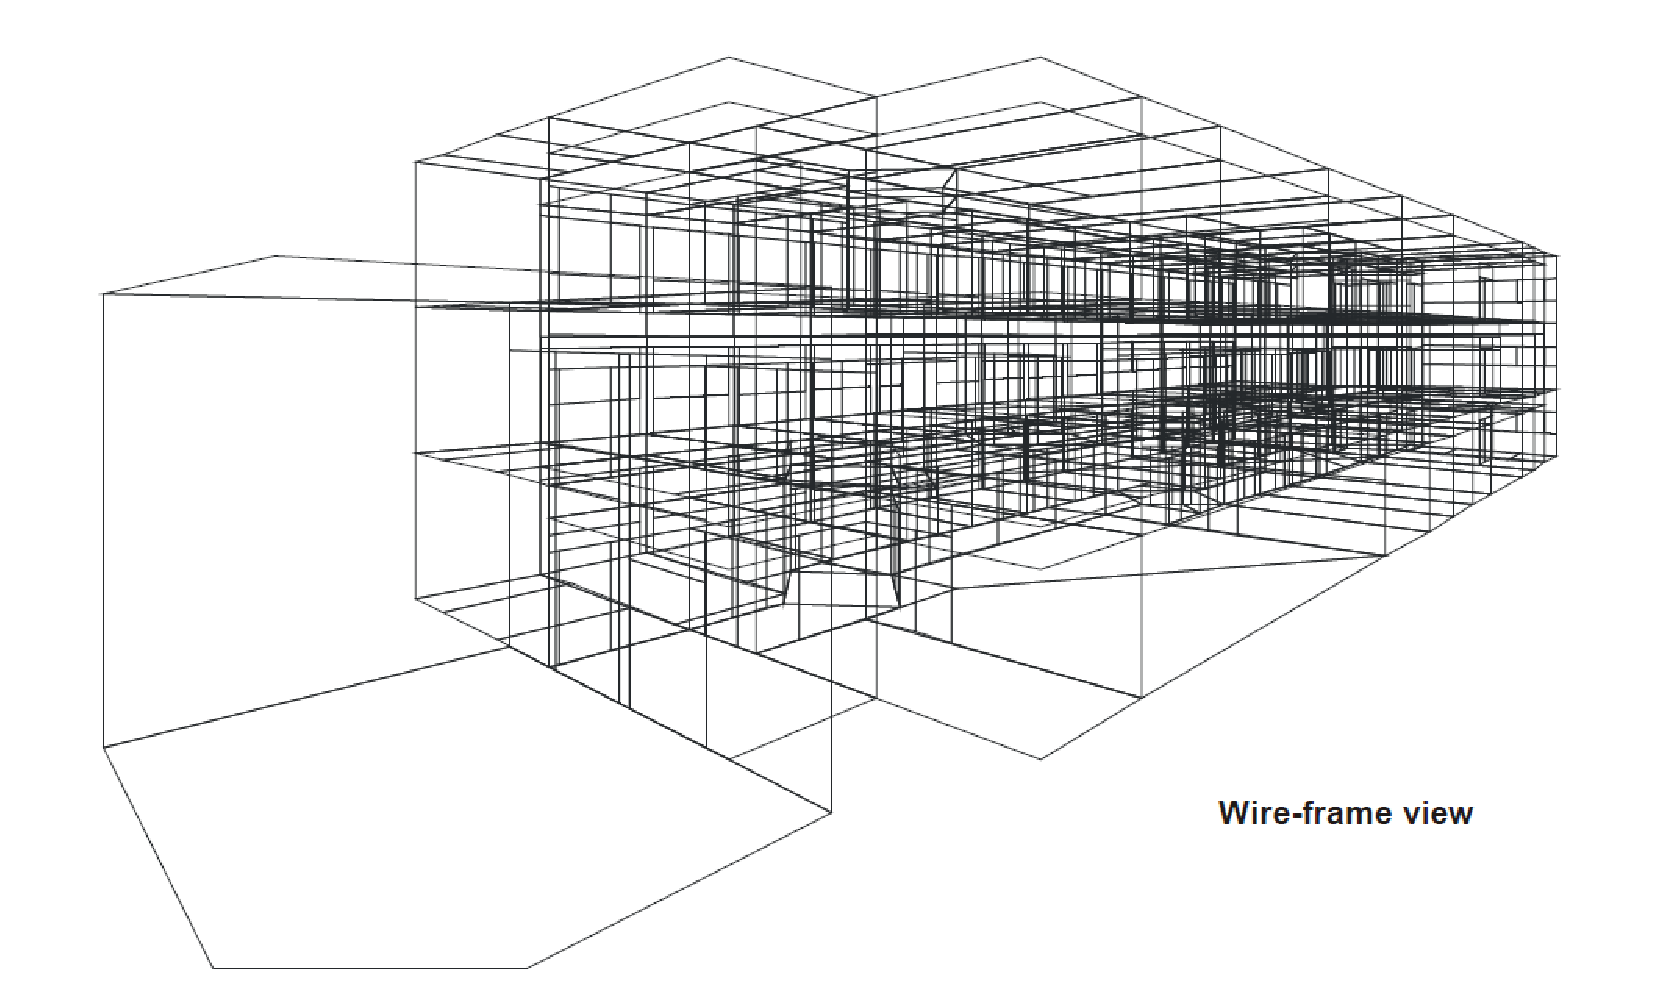
\includegraphics[width=14cm]{FrontPage}
	\center{Sometimes the reactive near-field area becomes even harder to model}
	\vspace*{2cm}
    
	Aalborg University\\
	P9, Autumn Semester 2014\\
	Wireless Communication Systems\\
\end{center}
	\cleardoublepage
	This paper is the documentation of the work related to the mini-project done in the first part of the course \textit{Multi-Agent Radio Communication}. These mini-project and exercises have been solved and documented as a team effort of the course participants.\\

The group consists of:
	\begin{description}
	\item \hspace{4cm} Jesper Nysted Andersen
 	\item \hspace{4cm} Maria Stefan
 	\item \hspace{4cm} Anders Karstensen
 	\item \hspace{4cm} Maria Carmela Cascino
 	\item \hspace{4cm} Johannes Hejselbæk
 	\item \hspace{4cm} Juan Alberto Cabrera Guerrero
 	\item \hspace{4cm} Djamschid Safi
 	\item \hspace{4cm} Pablo Fuentes
	\end{description}

\vspace{2cm}
The documentation is divided into chapters corresponding to the different exercises of the mini project.
	%\cleardoublepage
	\pagestyle{plain}
		
%%%%% Table of content %%%%%
	\tableofcontents 
	\onehalfspacing
	\pagestyle{fancy} % Normal pagesetup with page numbering (change to plain to remove header)
	\pagenumbering{arabic} 
    \setcounter{page}{0} % Sætter sidetal til 1
%%%%% START OF DOCUMENT  %%%%%	

\part{Patrick Part 1}

\chapter{MM1 - Time reversal techniques}
In this mini module we are going to simulate the designed Yagi antenna using both ADS and CST in the frequency domain. 
\section{Problem A}
\textit{Calculate the delay spread for this channel model using the average power delay profile.}
\section{Problem B}
\textit{MINIMISING RADIATED POWER. For the same given coverage area, compare the radiated power (interference) of a single antenna system, $P_{tx}^1$, to the total radiated power of an M-antenna distributed system, $P_{tx}^M$, for both the network (downlink) and the portable side (uplink). State the implications of the relation.}\\

In this "lemma" we need to consider these two cases: Single Antenna System (S) and M Antenna Distributed System (M).
For the case of Single Antenna System, as there is only one antenna, the total area covered ($A^s_C$) is the area covered for the single antenna.
\begin{equation}
A^s_c = \pi \cdot (d^s_{c})^2
\end{equation}

For that area the path loss has the expression:
\begin{equation}
PL^s_{max} = \dfrac{P^s_{R}}{P_{d_{c}}} = c\left(\dfrac{A^s_c}{\pi}\right)^{\frac{\varphi}{2}}= c\left(d^s_c\right) ^{\varphi}
\end{equation}

Note that in the last expression $P_{d_{c}}$ has no superscript, given that is the minimum acceptable downlink power level and must be considered with the same value in the Distributed System case. Nonetheless, the area covered by each antenna in the DS is smaller, so the power that the antenna needs to reach $P_{d_{c}}$ at the cell bounding will be lower.\\

In order to compute the transmitted power let's take into account the expression of the cover area for the M Antenna System:
\begin{align*}
A^m_{c,total} &= M \cdot A^m_{c} \\
&= M \cdot \pi \cdot (d^m_{c})^{2}
\end{align*}

Comparing it with the area covered in the single antenna case we obtain the relation between the radius:
\begin{equation}
A^s_{c}= A^m_{Tc}\ \ \Longrightarrow \ \ \pi \cdot (d^s_{c})^2 = M \cdot \pi \cdot (d^m_{c})^2 \ \  \Longrightarrow \ \
\frac{(d^s_{c})^2}{M} = (d^m_{c})^2
\end{equation}

Next step is to find the relation between the path loss in the two cases:
\begin{align*}
PL^m_{max} &= c(d^m_c) ^{\varphi} \\
	&= c(d^s_c)^{\varphi}\cdot (M)^{\frac{-\varphi}{2}}\\ %Shit
&\Downarrow\\	
	PL^m_{max} &= PL^s_{max} \cdot (M)^{\frac{-\varphi}{2}}
\end{align*}

As the $P_{d_{c}}$ is the same in both cases we can obtain the relation between the power received in both cases at the reference distance (1m):
\begin{align*}
\frac{P^s_R}{PL^s_{max}}=\frac{P^m_R}{PL^m_{max}}\ \ &\Longrightarrow \ \ P^m_R = P^s_R \cdot (M)^{\frac{-\varphi}{2}}
\end{align*}

Finally, to study the radiated power we have to distinguish the downlink from the uplink. In the \textbf{uplink} we consider the power needed for the user to connect to the antenna:
\begin{align*}
P^M_{tx} &= P^1_{tx} \cdot M^{\frac{-\varphi}{2}}
\end{align*}
\textit{For any value of $\varphi$ the Multi-antenna distributed system is more efficient than the Single Antenna System}\\

In the \textbf{downlink} scenario, the total radiated power is the sum of the radiated power for each antenna:
\begin{align*}
P^M_{tx} &= P^1_{tx} \cdot M^{\frac{-\varphi}{2}} \cdot M\\
&=P^1_{tx} \cdot M^{\frac{2-\varphi}{2}}
\end{align*}
\textit{It can be obtained from this expression that for values of path loss exponent ($\varphi$) higher than 2, the Distributed System is more efficient.}
\section{Problem C}
\textit{REDUCING MAXIMUM PATH LOSS. For the same given coverage area, compare the maximum path loss of a single antenna system, $PL_{max^1}$, to the maximum path loss of an M-antenna distributed system, $PL_{max^M}$, and express the reduction in the dynamic range. Define path loss at the cell boundary, $d_c$, of the single-antenna system (as in the boxed expression above). State the implications of the relation.}\\

The maximum pathloss is given by:
\begin{flalign}
&& PL_{max} \equiv & \frac{P_R}{P_{d_c}} = C\left(\frac{A_c}{\pi}\right)^{\sfrac{\gamma}{2}} & \label{eq:MaximumPathLoss}
\end{flalign}  

where $PL_{max}$ is the maximum pathloss, $P_R$ is the reference power which is equivalent to the transmitted power and $P_{d_c}$ is the minimum acceptable downlink power level at the cell boundary which is at the distance $d_c$ from the cell center (Radius of coverage area). $A_c$ is the coverage area of the cell and $\gamma$ is the pathloss exponent. C is a scaling constant. \\

From \equref{eq:MaximumPathLoss} it can be seen that there is a direct relation to the area of the cell. Therefore the relation between number of antennas ($M$) and the area ($A_c$) found in \secref{sec:mm3_PbA} and shown in \equref{eq:ExpressionForAcWithM} can be used here. 


\section{Problem D}
\textit{ UPLINK $C/I$ (NOISE INGRESS). For the same given coverage area, compare the minimum $C/I$ of a single 
antenna system, $(C/I)^1$, to the minimum $C/I$ of an M-antenna distributed system, $(C/I)^M$, assuming a "distant 
interferer" received at power level I. Derive the expression for $(C/I)^M$ for the case with transmit power 
reduction at the portable (see (b)).}

Noise ingress in the leaking in of a signal when electrical energy enters a coaxial environment. 
\section{Problem E}
\textit{Perform time reversal in a MISO context for each set of 2 channel realizations (one from A and one from D). Calculate the average power delay profile of the equivalent channel and from that the delay spread. How does it compare to the delay spread calculated in B and C?}

\chapter{MM2 - Spatial data multiplexing and space-time coding}
In this mini module we are going to simulate the designed Yagi antenna using both ADS and CST in the frequency domain. 
\section{Problem C}
\section{Problem 2}
\textit{To waterfill or not?}

\textit{Consider a 2x2 MIMO channel with ZMCSCG elements with unit variance. Develop your code for a square MIMO system of arbitrary number of antennas (and not just 2) since you will need it later in the problem. How does channel knowledge affect the Ergodic Capacity and the 10 percent Outage Capacity at low and high SNR values.} \\

\textit{Now increase the number of antennas to 4, 6 and 8 (remember the system is still MxM). How does channel knowledge affect ergodic capacity at 10 dB SNR with an increase in the number of antennas.}

ZMCSCG stands for Zero-Mean Circulant Symmetric Complex Gaussian. \\

Using multiple transmit and receive antennas will help increase the capacity of the MIMO system. This can be seen from the capacity values obtained in Matlab, where the capacity formula is $C=C+log_{2}(1+SNR \lambda ^{2})$. The channel capacity is also higly related to the correlation between transmit and receive antennas. The capacity is reduced as the correlation becomes higher. .......\\

Another statistical notion of the channel capacity is the outage channel capacity. It is defined as $P_{out}(R)=Pr(C(H)<R)$. 

The maximum outage capacity can be defined as the maximum rate that can be maintained in all channel states with some probability of outage (no data transmission).

\section{Multiplexing question 1}
\textit{From the expression of the MIMO channel capacity in terms of the normalized channel transfer matrix H \equref{eq:1_multiplexing}, derive the expression of the capacity in terms of the singular values l of H \equref{eq:2_multiplexing}.
Hint : remember how $H$ is decomposed - expand}
\begin{flalign}
 && C =& log_{2}\left(det\left(I + \frac{\rho}{M}HH^{H}\right) \right) & \label{eq:1_multiplexing}\\
\end{flalign}
The channel transfer matrix H can be expressed with the singular value decompression as 
\begin{flalign}
 && H =&  SUV^{H} &
\end{flalign}
where $S$ and $V$ are unitary matrices and $S$ the diagonal matrix containing the singular values of $H$. Inserting this into \equref{eq:1_multiplexing} the formula can be rearranged.
\begin{flalign}
 &&  C =& log_{2}\left(det\left(I + \frac{\rho}{M}SUV^{H}VU^{H}S^{H}\right) \right) & \\
 &&  =& log_{2}\left(det\left(I + \frac{\rho}{M}SUU^{H}S^{H}\right) \right) & 
 \end{flalign}
Expanding with $SS^{H}$
 \begin{flalign} 
 &&  C =& log_{2}\left(det\left[SS^{H}\left(I + \frac{\rho}{M}SUU^{H}S^{H}\right)SS^{H}\right] \right) & \\
 &&  =& log_{2}\left(det\left[S\left(I + \frac{\rho}{M}UU^{H}\right)S^{H}\right] \right) & \\
 &&  =& log_{2}\left(det\left(S\right)det\left(I + \frac{\rho}{M}UU^{H}\right)det\left(S^{H}\right) \right) & \\
 &&  =& log_{2}\left(det\left(SS^{H}\right)det\left(I + \frac{\rho}{M}UU^{H}\right) \right) & \\
 &&  =& log_{2}\left(det\left(I + \frac{\rho}{M}UU^{H}\right) \right) &
 \end{flalign}
 Where $U = diag(\lambda_i)$, with $\lambda_i=0$ for $i>rank(U)=rank(H)$
 
 \begin{flalign}
 &&  C =& log_{2}\left(det\left(I + \frac{\rho}{M}diag\left(\lambda^{2}_{i}\right)\right) \right) & \\
 &&  =& log_{2}\left(diag\left(1 + \frac{\rho}{M}\lambda^{2}_{i}\right)\right) & \\
 && =& log_{2}\left(\prod_{i = 1}^{k}\left(1 + \frac{\rho}{M}\lambda^{2}_{i}\right)\right) & \\
 && =& \sum_{i = 1}^{k}log_{2}\left(1 + \frac{\rho}{M}\lambda^{2}_{i}\right) & \label{eq:2_multiplexing}
\end{flalign}

\section{Problem D}

\part{Troels Part 1}

\chapter{MM3 - Distributed antenna systems}
In this mini module we are going to simulate the designed Yagi antenna using both ADS and CST in the frequency domain. 
\section{Problem A}
\textit{Calculate the delay spread for this channel model using the average power delay profile.}
\section{Problem B}
\textit{MINIMISING RADIATED POWER. For the same given coverage area, compare the radiated power (interference) of a single antenna system, $P_{tx}^1$, to the total radiated power of an M-antenna distributed system, $P_{tx}^M$, for both the network (downlink) and the portable side (uplink). State the implications of the relation.}\\

In this "lemma" we need to consider these two cases: Single Antenna System (S) and M Antenna Distributed System (M).
For the case of Single Antenna System, as there is only one antenna, the total area covered ($A^s_C$) is the area covered for the single antenna.
\begin{equation}
A^s_c = \pi \cdot (d^s_{c})^2
\end{equation}

For that area the path loss has the expression:
\begin{equation}
PL^s_{max} = \dfrac{P^s_{R}}{P_{d_{c}}} = c\left(\dfrac{A^s_c}{\pi}\right)^{\frac{\varphi}{2}}= c\left(d^s_c\right) ^{\varphi}
\end{equation}

Note that in the last expression $P_{d_{c}}$ has no superscript, given that is the minimum acceptable downlink power level and must be considered with the same value in the Distributed System case. Nonetheless, the area covered by each antenna in the DS is smaller, so the power that the antenna needs to reach $P_{d_{c}}$ at the cell bounding will be lower.\\

In order to compute the transmitted power let's take into account the expression of the cover area for the M Antenna System:
\begin{align*}
A^m_{c,total} &= M \cdot A^m_{c} \\
&= M \cdot \pi \cdot (d^m_{c})^{2}
\end{align*}

Comparing it with the area covered in the single antenna case we obtain the relation between the radius:
\begin{equation}
A^s_{c}= A^m_{Tc}\ \ \Longrightarrow \ \ \pi \cdot (d^s_{c})^2 = M \cdot \pi \cdot (d^m_{c})^2 \ \  \Longrightarrow \ \
\frac{(d^s_{c})^2}{M} = (d^m_{c})^2
\end{equation}

Next step is to find the relation between the path loss in the two cases:
\begin{align*}
PL^m_{max} &= c(d^m_c) ^{\varphi} \\
	&= c(d^s_c)^{\varphi}\cdot (M)^{\frac{-\varphi}{2}}\\ %Shit
&\Downarrow\\	
	PL^m_{max} &= PL^s_{max} \cdot (M)^{\frac{-\varphi}{2}}
\end{align*}

As the $P_{d_{c}}$ is the same in both cases we can obtain the relation between the power received in both cases at the reference distance (1m):
\begin{align*}
\frac{P^s_R}{PL^s_{max}}=\frac{P^m_R}{PL^m_{max}}\ \ &\Longrightarrow \ \ P^m_R = P^s_R \cdot (M)^{\frac{-\varphi}{2}}
\end{align*}

Finally, to study the radiated power we have to distinguish the downlink from the uplink. In the \textbf{uplink} we consider the power needed for the user to connect to the antenna:
\begin{align*}
P^M_{tx} &= P^1_{tx} \cdot M^{\frac{-\varphi}{2}}
\end{align*}
\textit{For any value of $\varphi$ the Multi-antenna distributed system is more efficient than the Single Antenna System}\\

In the \textbf{downlink} scenario, the total radiated power is the sum of the radiated power for each antenna:
\begin{align*}
P^M_{tx} &= P^1_{tx} \cdot M^{\frac{-\varphi}{2}} \cdot M\\
&=P^1_{tx} \cdot M^{\frac{2-\varphi}{2}}
\end{align*}
\textit{It can be obtained from this expression that for values of path loss exponent ($\varphi$) higher than 2, the Distributed System is more efficient.}
\section{Problem C}
\textit{REDUCING MAXIMUM PATH LOSS. For the same given coverage area, compare the maximum path loss of a single antenna system, $PL_{max^1}$, to the maximum path loss of an M-antenna distributed system, $PL_{max^M}$, and express the reduction in the dynamic range. Define path loss at the cell boundary, $d_c$, of the single-antenna system (as in the boxed expression above). State the implications of the relation.}\\

The maximum pathloss is given by:
\begin{flalign}
&& PL_{max} \equiv & \frac{P_R}{P_{d_c}} = C\left(\frac{A_c}{\pi}\right)^{\sfrac{\gamma}{2}} & \label{eq:MaximumPathLoss}
\end{flalign}  

where $PL_{max}$ is the maximum pathloss, $P_R$ is the reference power which is equivalent to the transmitted power and $P_{d_c}$ is the minimum acceptable downlink power level at the cell boundary which is at the distance $d_c$ from the cell center (Radius of coverage area). $A_c$ is the coverage area of the cell and $\gamma$ is the pathloss exponent. C is a scaling constant. \\

From \equref{eq:MaximumPathLoss} it can be seen that there is a direct relation to the area of the cell. Therefore the relation between number of antennas ($M$) and the area ($A_c$) found in \secref{sec:mm3_PbA} and shown in \equref{eq:ExpressionForAcWithM} can be used here. 


\section{Problem D}
\textit{ UPLINK $C/I$ (NOISE INGRESS). For the same given coverage area, compare the minimum $C/I$ of a single 
antenna system, $(C/I)^1$, to the minimum $C/I$ of an M-antenna distributed system, $(C/I)^M$, assuming a "distant 
interferer" received at power level I. Derive the expression for $(C/I)^M$ for the case with transmit power 
reduction at the portable (see (b)).}

Noise ingress in the leaking in of a signal when electrical energy enters a coaxial environment. 


\part{Patrick Part 2}

\chapter{MM4 - Advantages of using directive antennas (SDMA)}
In this mini module we are going to simulate the designed Yagi antenna using both ADS and CST in the frequency domain. 
\section{Problem A}
\textit{Calculate the delay spread for this channel model using the average power delay profile.}
\subsection{Question 2}
\textit{The user and interferer are now replaced by angular distribution of: Cs($\Phi$)= 1 within 80 to 100 deg. , 0 outside and Is($\Phi$)=3/4 within 54 to 67 deg., 0 outside}

\subsubsection{a) what is the peak to null depth for the measured response of the user compared to max and sidelobe}

To answer this question we need to find the azimuthal measurement response. This is done finding the correlation function between the environment as a function of $\varphi$, and the antenna pattern as shown in \equref{eq:effective}.

\begin{flalign}
&&	m(\varphi) =& \oint e(\Phi) \cdot a(\Phi - \varphi)d\Phi =R_{e,a^{*}}(\varphi)	 &\label{eq:effective}
\end{flalign}

The resulting pattern is shown in \textbf{FIGURE}. From which, graphically, the peak to null depth can be calculated  \textbf{PUT THE CALCULATED RESULT}

\subsubsection{b) What is the Cs/Is of the measured responses and what direction will the response function be centered at if performing a sweep (radar scan) with the antenna on the user and on the interferer?}

This value can be computed by two different methods. One is to integrate the product of the antenna pattern and the angular distribution of the users over the whole circle as shown in \equref{eq:bruteforce}.

\begin{flalign}
&&	\frac{Cs}{Is} =& \frac{\oint C(\varphi)\cdot a(\varphi)d\varphi}{\oint I(\varphi)\cdot a(\varphi)d\varphi}	 &\label{eq:bruteforce}
\end{flalign}

Another method to compute this result is to use the azimuthal measurement response of both, the user and the interferer. In the previous question, the graph of the $m_{C}(\varphi)$ was shown and in figure INSERT FIGURE $m_{I}(\varphi)$ we show this response for the interferer in \textbf{FIGURE}.

Mathematically, performing a sweep (radar scan) is equivalent to find the correlation function described in \equref{eq:effective}. Due to the properties of this ``convolution'', the user (whose mean is located at 90 degrees) will be shifted $90 + 90$ degrees. As seen in \textbf{FIGURE}. The interferer, because of the same argument, will be shifted $60.5 + 60.5$ degrees.

In order to compute this result by this second method, we need to calculate the $Cs$ and the $Is$ using $m_{C}(\varphi)$ and $m_{I}(\varphi)$. This is done considering the user as a single source in $m_{C}(\varphi)$ at 180 degrees and the interferer as a single source in $m_{I}(\varphi)$ at 121 degrees. \textbf{MAYBE EXPAND THIS EXPLANATION}
\section{Problem B}
\textit{MINIMISING RADIATED POWER. For the same given coverage area, compare the radiated power (interference) of a single antenna system, $P_{tx}^1$, to the total radiated power of an M-antenna distributed system, $P_{tx}^M$, for both the network (downlink) and the portable side (uplink). State the implications of the relation.}\\

In this "lemma" we need to consider these two cases: Single Antenna System (S) and M Antenna Distributed System (M).
For the case of Single Antenna System, as there is only one antenna, the total area covered ($A^s_C$) is the area covered for the single antenna.
\begin{equation}
A^s_c = \pi \cdot (d^s_{c})^2
\end{equation}

For that area the path loss has the expression:
\begin{equation}
PL^s_{max} = \dfrac{P^s_{R}}{P_{d_{c}}} = c\left(\dfrac{A^s_c}{\pi}\right)^{\frac{\varphi}{2}}= c\left(d^s_c\right) ^{\varphi}
\end{equation}

Note that in the last expression $P_{d_{c}}$ has no superscript, given that is the minimum acceptable downlink power level and must be considered with the same value in the Distributed System case. Nonetheless, the area covered by each antenna in the DS is smaller, so the power that the antenna needs to reach $P_{d_{c}}$ at the cell bounding will be lower.\\

In order to compute the transmitted power let's take into account the expression of the cover area for the M Antenna System:
\begin{align*}
A^m_{c,total} &= M \cdot A^m_{c} \\
&= M \cdot \pi \cdot (d^m_{c})^{2}
\end{align*}

Comparing it with the area covered in the single antenna case we obtain the relation between the radius:
\begin{equation}
A^s_{c}= A^m_{Tc}\ \ \Longrightarrow \ \ \pi \cdot (d^s_{c})^2 = M \cdot \pi \cdot (d^m_{c})^2 \ \  \Longrightarrow \ \
\frac{(d^s_{c})^2}{M} = (d^m_{c})^2
\end{equation}

Next step is to find the relation between the path loss in the two cases:
\begin{align*}
PL^m_{max} &= c(d^m_c) ^{\varphi} \\
	&= c(d^s_c)^{\varphi}\cdot (M)^{\frac{-\varphi}{2}}\\ %Shit
&\Downarrow\\	
	PL^m_{max} &= PL^s_{max} \cdot (M)^{\frac{-\varphi}{2}}
\end{align*}

As the $P_{d_{c}}$ is the same in both cases we can obtain the relation between the power received in both cases at the reference distance (1m):
\begin{align*}
\frac{P^s_R}{PL^s_{max}}=\frac{P^m_R}{PL^m_{max}}\ \ &\Longrightarrow \ \ P^m_R = P^s_R \cdot (M)^{\frac{-\varphi}{2}}
\end{align*}

Finally, to study the radiated power we have to distinguish the downlink from the uplink. In the \textbf{uplink} we consider the power needed for the user to connect to the antenna:
\begin{align*}
P^M_{tx} &= P^1_{tx} \cdot M^{\frac{-\varphi}{2}}
\end{align*}
\textit{For any value of $\varphi$ the Multi-antenna distributed system is more efficient than the Single Antenna System}\\

In the \textbf{downlink} scenario, the total radiated power is the sum of the radiated power for each antenna:
\begin{align*}
P^M_{tx} &= P^1_{tx} \cdot M^{\frac{-\varphi}{2}} \cdot M\\
&=P^1_{tx} \cdot M^{\frac{2-\varphi}{2}}
\end{align*}
\textit{It can be obtained from this expression that for values of path loss exponent ($\varphi$) higher than 2, the Distributed System is more efficient.}

%%%%% REFERENCES %%%%%%
\part{References}
\chapter{List of references}  \label{ch:reflist}
	Figures and tables are produced by the project group unless otherwise specified.
\begingroup  
  \let\chapter\section 
  \makeatletter\let\markboth\@firstoftwo\makeatother 
  \pagestyle{plain}
  \listoffigures 
  \listoftables
	\bibliographystyle{apalike}
   \begin{flushleft}
    \bibliography{references}
   \end{flushleft} 
  \pagestyle{fancy}
\endgroup


%%%%% NOTES %%%%%
\chapter{NOTES AND STUFF}

This appendix is for the group members to see how to code basic \LaTeX{} functions.
%%%%%%%%%%%%%%%%%%%%%%%%%%%%%%%%%%%%%%%%%%%%%%%%%%%%%%%%%%%%%%%%%%%%%%%%%%%%%%%%%%%%%%%%%%%%%%%%%%%%%
\section{Insert a figures/picture}
Remember that you need to convert to .eps if the picture to a vectorpicture before you upload it to the image folder in the svn drive. This can be done using \url{www.go2convert.com}.\\ % <- these \\ means newline

The code for including the figure is listed here:

\begin{figure}[!h]
  \centering
  \includegraphics[width=4cm]{2rayModel.eps}
  \caption{Sample image.}
  \label{fig:REMEMBER_TO_CHANGE_THE_LABEL}
\end{figure}

When you need to write about the figure do like this: In \figref{fig:REMEMBER_TO_CHANGE_THE_LABEL} you see a sample image. The size of this can be set with the width=?? bracket.

This is a shot code for a figure:
\fig[keepaspectratio=true,width=4cm]{2rayModel.eps}{Sample image.}{fig:REMEMBER_TO_CHANGE_THE_LABEL2}

%%%%%%%%%%%%%%%%%%%%%%%%%%%%%%%%%%%%%%%%%%%%%%%%%%%%%%%%%%%%%%%%%%%%%%%%%%%%%%%%%%%%%%%%%%%%%%%%%%%%%
\section{Making a list}

To make a list with points do like this:
\begin{pitemize}
\item $P_{TX}$: Note the greenstuf in the code for this line, this is how you do math
\item Another point
\end{pitemize}

With numbers:
\begin{penumrate}
\item $P_{TX}$: Note the greenstuf in the code for this line, this is how you do math
\item Another point
\end{penumrate}

%%%%%%%%%%%%%%%%%%%%%%%%%%%%%%%%%%%%%%%%%%%%%%%%%%%%%%%%%%%%%%%%%%%%%%%%%%%%%%%%%%%%%%%%%%%%%%%%%%%%%
\section{How to write math}
If one is to write normal math expression inline then just use the dollar $style$. If you need a equation then use the following:

\begin{flalign}
&&	c_{i} =& \frac{\sum \sqrt{\left(X_{i}-X_{j}\right)^{2}+\left(Y_{i}-Y_{j}\right)^{2}}}{\sum h_{i}}	& [\SI{}{\meter}] &\label{eq:REMEMBER_TO_CHANGE_THE_LABEL3} \\
&&	dist_{ij} =& \frac{(t_4-t_1)-(t_3-t_2)}{2} \cdot v	& [\SI{}{\meter}] & \label{eq:REMEMBER_TO_CHANGE_THE_LABEL4}
\end{flalign}

The when you need to make a references to the equation you can just do like this: In \equref{eq:REMEMBER_TO_CHANGE_THE_LABEL3} it is seen that... And in \equref{eq:REMEMBER_TO_CHANGE_THE_LABEL4} it is seen that... \\

It is important always to use the right SI-unit (See: \secref{sec:SIunit}) ! Mark this in the last bracket\\
Remember not to remove the \texttt{\&} symbols in the code, these control the spacing. 

%%%%%%%%%%%%%%%%%%%%%%%%%%%%%%%%%%%%%%%%%%%%%%%%%%%%%%%%%%%%%%%%%%%%%%%%%%%%%%%%%%%%%%%%%%%%%%%%%%%%%
\section{Use the right SI-unit} \label{sec:SIunit}
We are engineers and therefore we only use correct SI-units. This is easy in \LaTeX{} as there is a function for this and it works all over. You do like this:\\

If we need to write something in meters then do this: \SI{10,00}{\meter} or \SI{10.00}{\meter}, as seen in the code first bracket is the number, and you can use dot or comma it will be correct in the pdf as the SI function controls this.  Some other examples: \SI{0.01}{\micro\watt} / \SI{250}{\milli\watt} / \SI{285.517}{\milli\meter} / \SI{2100}{\mega\hertz} /\SI{}{\decibelm}. Lastly here is one where we have the per symbol and want i ``pretty'' as you know i like; \SIf{}{\meter\per\second} otherwise it will be; \SI{}{\meter\per\second}

%%%%%%%%%%%%%%%%%%%%%%%%%%%%%%%%%%%%%%%%%%%%%%%%%%%%%%%%%%%%%%%%%%%%%%%%%%%%%%%%%%%%%%%%%%%%%%%%%%%%%
\section{Use references wisely} \label{sec:refs}
When working in latex one of the most important features is that references is generic. Therefore it is important to use these correct. We are using the labels to reference to this and as you may have notice in the code the first part of the label refers to what the label is attached to. eg. ``sec:'' for a section and ``eq:'' for a equation. We use different references as to where it is used and to what it refers, here is some examples:\\

(See \chref{ap:basiclatex}) will give you ``See chapter A'' \\ % yes it should be {ch:something} but i just use the other label as a exampel here.
(See \secref{sec:SIunit}) will give you ``See section A.4 (p.13)'' \\
(See \figref{fig:REMEMBER_TO_CHANGE_THE_LABEL2}) will give you ``See figure A.2 (p.12)'' \\
(See \equref{eq:REMEMBER_TO_CHANGE_THE_LABEL4}) will give you ``See equation A.2 (p.13)'' \\
(See \apref{ap:basiclatex}) will give you ``See appendix A (p.12)'' \\

And as you may already notice this change as the document evolves and therefore what I have put in with hardcode is already wrong. But the generic code using the correct labels and ref-types is always referring to the correct place.\\

If you need to make a reference to something and there is no label yet, then always put it on the chapter/section header or similar as this is then the place all of us can look for it. Good practice is always to make a label then others can use this even if you do not need it yourself.

%%%%%%%%%%%%%%%%%%%%%%%%%%%%%%%%%%%%%%%%%%%%%%%%%%%%%%%%%%%%%%%%%%%%%%%%%%%%%%%%%%%%%%%%%%%%%%%%%%%%%
\section{Making a table} 
\ptable{| p{10cm} | p{8cm} |}{ %
Property 							&	Description 												\\ \hline
Gain of received power 		        &	$G_r = 1$											        \\ \hline
Gain of transmitted power 	        &	$G_t  =  1$										            \\ \hline
Frequency							&	\textit{f} in \SI{}{\hertz}	    							\\ \hline
Propagation speed of signal			& 	$c$ in \SIf{}{\meter\per\second}                            \\ \hline	
Power transmitted 			        &	$P_{t(dBm)}$ in \SI{}{\decibelm} 	                        \\ \hline
}{Free-Space Model properties}{tab:environment}

The properties needed to define the Free-Space Model is listed in \tref{tab:environment}.  

\section{How to insert Matlab code in latex}
We use the folder \texttt{code} in the SVN folder. Therefore latex can extract and display code in the worksheets without the need of copying anything. \\

An example of this is seen below:
\code{language=Matlab,caption = Friis propagation model,label=cl:envfreespace,linerange={1-8},firstnumber=1}{code/initPropaFriis.m}

Note that there is multiple parameters which have to be set: \\
language        = Matlab                          (The language of the code)                 \\
caption         = What ever the caption should be                                            \\
label           = cl:REMEMBER LABEL               (Give a unique label name)                 \\
linerange       = {1-8}              (Set the linerange of code you want to be shown)        \\
firstnumber     = 1                  (Set the first linenumber shown in the latex file)      \\

A reference to the code can be done like this; As seen in \cref{cl:envfreespace}...

\end{document}
